\begin{frame}{$\chi_{b1,2}(2,3P) \to \TwoS$ fit model}
\begin{columns}[T]
\column{.5\textwidth}
  \centering
  \setlength{\unitlength}{1mm}
  \begin{picture}(50,80)
      %
    \put(0,0){
      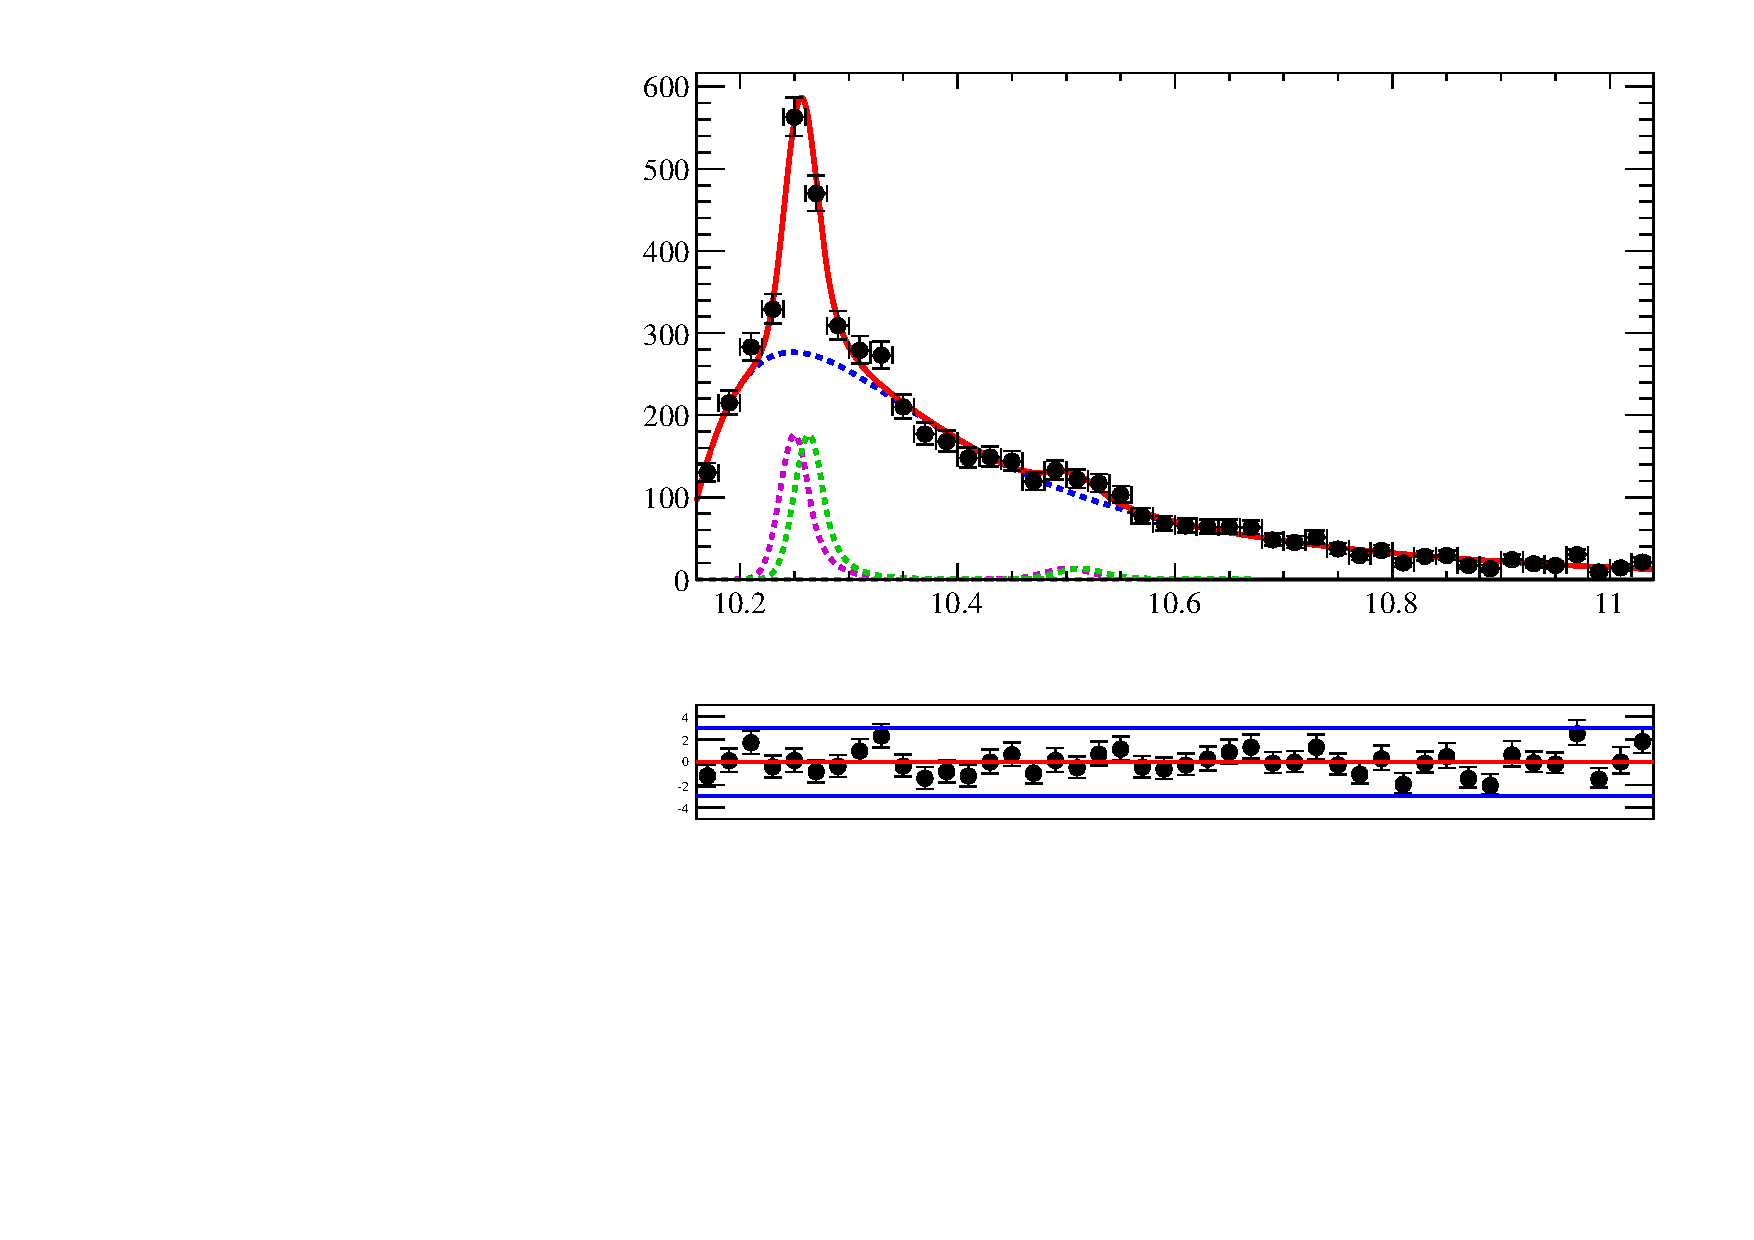
\includegraphics[width=50mm, height=40mm]{chib2s-fit/f2012_18_40}
    }
    
    \put(0,40){
      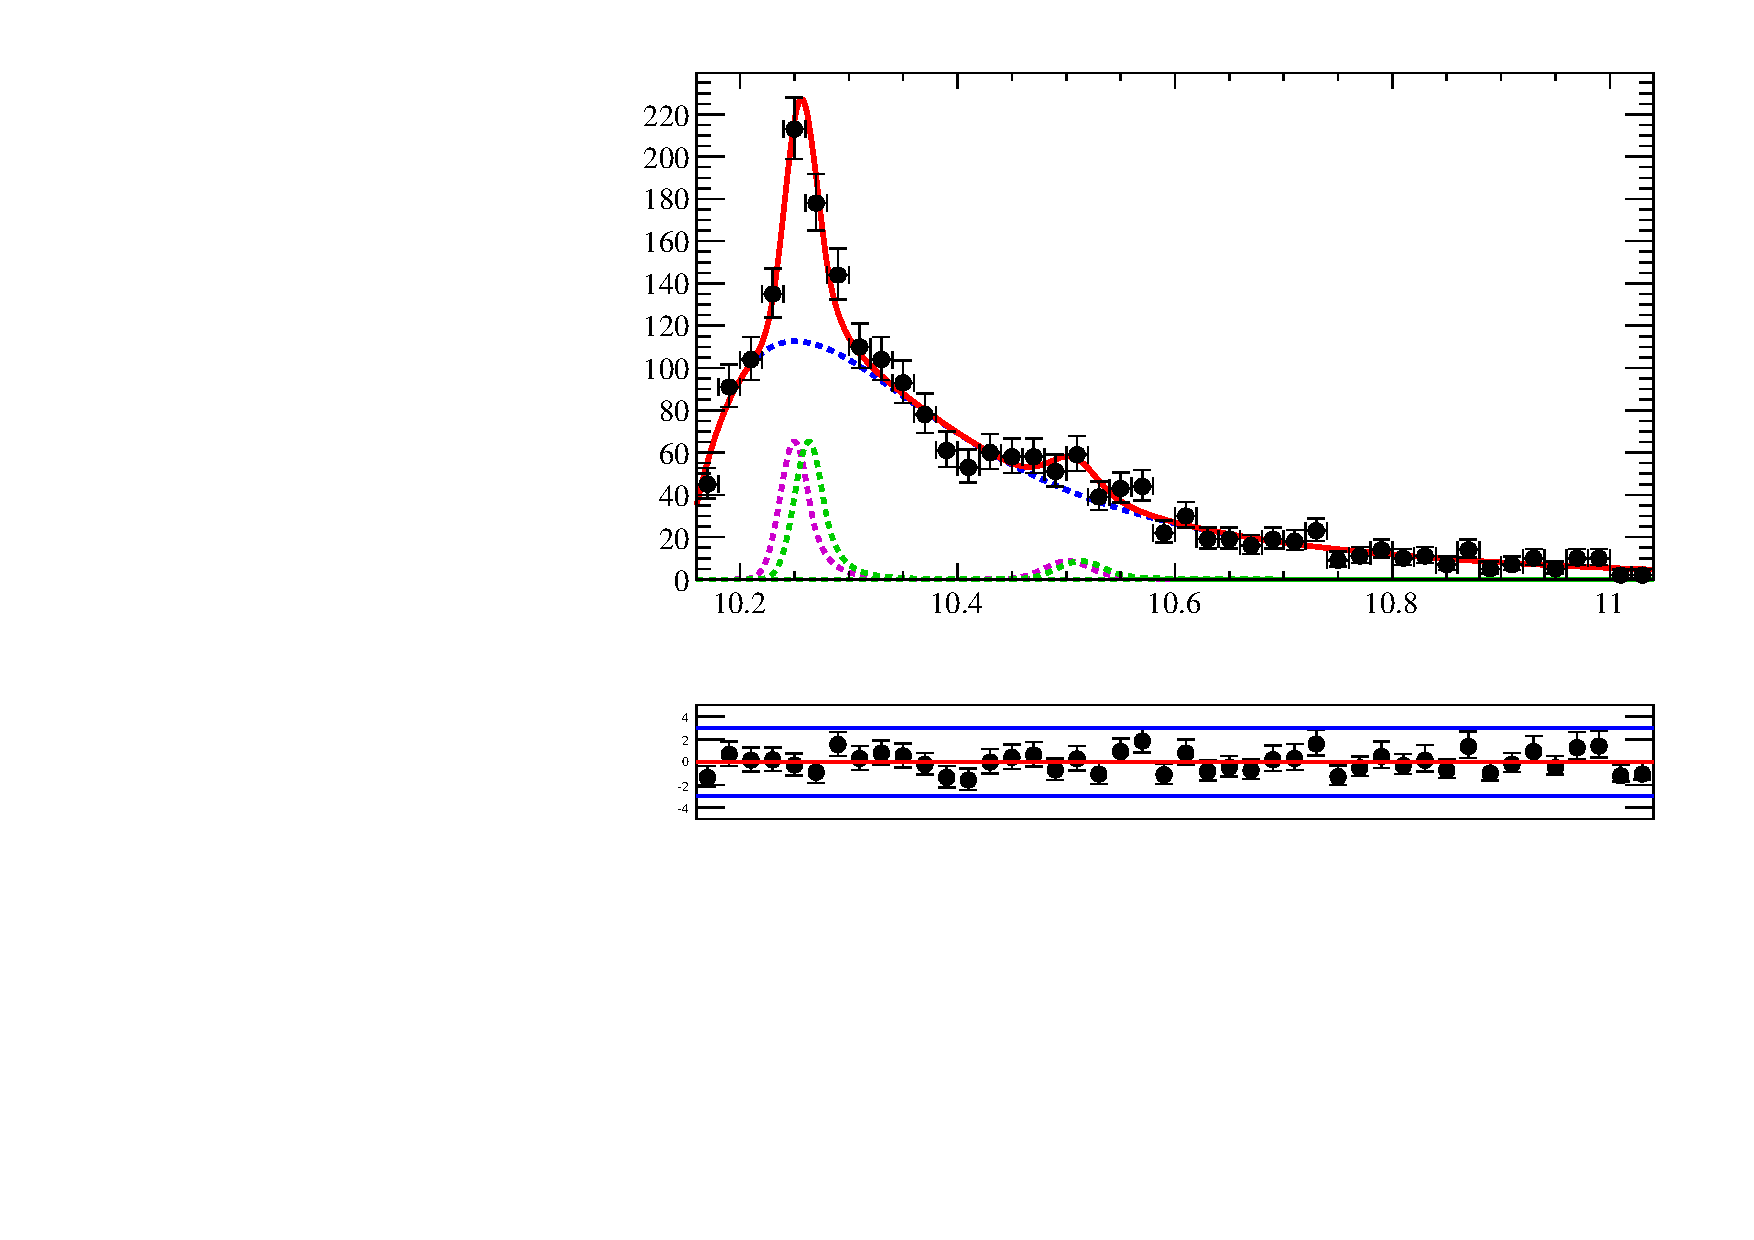
\includegraphics[width=50mm, height=40mm]{chib2s-fit/f2011_18_40}
    }

    \put(0,15){\tiny \begin{sideways}Candidates/(20\mevcc)\end{sideways}}
    \put(2,9){\tiny $m_{\mumu \gamma} - m_{\mumu} + m_{\Y2S}^{PDG} \left[\gevcc\right]$}
    \put(25,30){$\sqs=8 \tev$}
    \put(20,25){\tiny $ 18 < p_T^{\Y2S} < 40\gevc$}
    
    \put(0,55){\tiny \begin{sideways}Candidates/(20\mevcc)\end{sideways}}
    \put(2, 49){\tiny $m_{\mumu \gamma} - m_{\mumu} + m_{\Y2S}^{PDG} \left[\gevcc\right]$}
    \put(25,70){$\sqs=7 \tev$}
    \put(20,65){\tiny $18 < p_T^{\Y2S} < 40\gevc$}
    %\graphpaper[2](0,0)(50, 40)        
  \end{picture}
\column{.5\textwidth}
\begin{itemize}
\item 4 Crystal Ball function for each of $\chi_{b1,2}(2,3P)$ signal
\item Product of exponential and linear combination of polinomials  for combinatorial background.
\end{itemize}
\end{columns}
\end{frame}
